\section{Campo elettrostatico – Campo elettrico coulombiano}
Partendo dalle ipotesi:
\begin{itemize}
    \item \textbf{Elettrostatica} (cariche ferme, non in movimento)
    \item \textbf{Mezzo nella regione di studio}:
   Omogeneo, lineare, isotropo (stesse proprietà fisiche in ogni direzione).
\end{itemize}

\subsection{Legge sperimentale di Coulomb}
    \[
        \overline{F}_{q0} = \frac{1}{4\pi\epsilon}\frac{q\cdot q_0}{r^2}\hat{u}'
    \]
    Indica la forza agente su $q_0$ dovuta alla presenza di q.\\

    \textbf{Campo elettrostatico $\overline{E}_c(P)$}: è una \textbf{forza elettrica specifica} ovvero di natura elettrica e per unità di carica
    \[
        \overline{E}_c(P) := \lim_{q_0 \to 0} \frac{\overline{F}_{q_0}}{q_0} = \frac{1}{4\pi\epsilon}\frac{q}{r^2}\hat{u}
    \]
    Questo modello ha significato se ci si trova sufficientemente lontani dalla carica in quanto essendo un modello dipendente dalla distanza come $\frac{1}{r^2}$, se essa tende a 0, il campo tende a infinito.
    \[
        \overline{F}_{q0} = q_0 \vec{E_c}(t), \quad [E_c] = [V]
    \]

\subsection{Proprietà del campo elettrostatico}

1) Non è solenoidale.

2) È un campo conservativo:

\[
\oint_{l_c} \vec{E_c} \cdot \hat{t}\,dl = 0 \quad \forall l_c
\]

\paragraph{Teorema di Stokes (o del rotore)}:

\[
\oint_{\gamma} \vec{E} \cdot \vec{dl} = \int_S (\nabla \times \vec{E}) \cdot \vec{dS}
\]
\begin{center}
    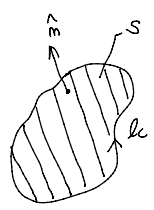
\includegraphics{immagini/image8.png}
\end{center}
a) $\partial S = l_c$\\
b) S non è unica\\
c) l'orientamento di S non si può scegliere a caso ma si ottiene a partire da $l_c$ con la regola della mano destra.\\

Applicando il teorema di Stokes:

\[
\oint_{l_c} \vec{E_c} \cdot \hat{t}\,dl = \int_S (\nabla \times \vec{E_c}) \cdot \hat{n}\,ds \quad \forall l_c
\]

Essendo l'integrale nullo per ogni $l_c$, il rotore del campo è nullo:

\[
\nabla \times \vec{E_c} = 0
\]

Il rotore è sempre nullo $\Rightarrow$ \textbf{campo irrotazionale}.

3) L'integrale di linea di $\vec{E_c}$ tra due punti $A$ e $B$ non dipende dal percorso:
\begin{center}
    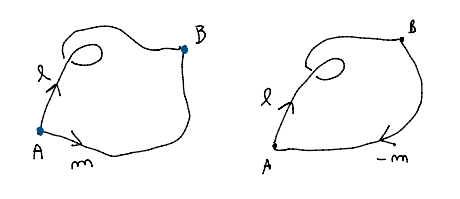
\includegraphics{immagini/image9.png}
\end{center}
\[
    \oint_{lc} \vec{E_c} \cdot \hat{t}dl = \int_{l} \vec{E_c} \cdot \hat{t}dl - \int_{m} \vec{E_c} \cdot \hat{t}dl
\]
\[
    \int_{l} \vec{E_c} \cdot \hat{t}dl = \int_{m} \vec{E_c} \cdot \hat{t}dl
\]
4) Proprietà del campo irrotazionale:

\[
\nabla \times (\nabla V) = 0, \quad \forall V \text{ scalare}
\]

Possiamo introdurre un \textbf{potenziale}: una variabile fisica ausiliare che serve a rappresentare una grandezza fisica che verifica implicitamente una legge.

\[
\nabla \times \vec{E_c} = 0
\]
ricordando che 
\[
    \vec{E_c} = -\nabla V
\]
Il campo scalare V è detto \textbf{potenziale elettrostatico}.\\
Trovando l'integrale di linea di $\vec{E_c}$ su l:

\[
\int_{A,l}^B \vec{E_c} \cdot \hat{t} dl = \int_{A,l}^B -\nabla V \cdot \hat{t} dl = V(A) - V(B)
\]
Questa soluzione deriva dal teorema del gradiente.

\subsection{Trovare V(P) da una singola carica puntiforme}

\begin{center}
    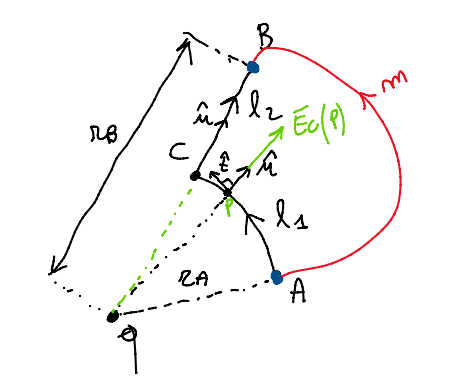
\includegraphics[scale = 0.7]{immagini/image10.png}
\end{center}

\[
\int_{A}^{B} \vec{E}_c \cdot \hat{t}  \, dl = \int_{A,l1}^{C} \vec{E}_c \cdot \hat{t}  \, dl + \int_{C,l2}^{B}\vec{E}_c \cdot \hat{t}  \, dl
\]

\[
\int_{A,l1}^{C} \vec{E}_c \cdot \hat{t}  \, dl = \int_{A,l1}^{C} \frac{q}{4 \pi \epsilon} \cdot \frac{1}{r^2_A} \cdot \hat{u} \cdot\hat{t}  \, dl = 0
\]

\[
\int_{C,l2}^{B} \vec{E}_c \cdot \hat{t}  \, dl = \int_{C,l2}^{B} |\vec{E}_c| \cdot \frac{\vec{E}_c}{|\vec{E}_c|} \cdot \hat{t}  \, dl = \int_{C}^{B} |\vec{E}_c|  \, dl = \int_{r_A}^{r_B} \frac{q}{4 \pi \epsilon} \cdot \frac{1}{r^2} dr = \frac{q}{4\pi\epsilon}(\frac{1}{r_A}-\frac{1}{r_B}) = V(A)-V(B)
\]

Imponendo le condizioni all'infinito
\[
\lim_{r\to\inf}V(P)=0 = \lim_{r\to\inf}(\frac{q}{4\pi\epsilon}\frac{1}{r} + c)  = 0+c = 0
\]

La D.D.P. non dipende dalla costante.\\
Nel momento in cui sono presenti più cariche si può sfruttare il principio di \textbf{sovrapposizione degli effetti}.\\

Non in elettrostatica si definisce l'analogo di $\vec{E}_c$ che è
\[
    \vec{E}(t,P) = \lim_{q_0\to 0}\frac{\vec{F}_{q0}(t,P)}{q_0}
\]
\[
    \vec{E}(t,P) = \vec{E}_c(t,P) + \vec{E}_i(t,P)
\]
Con $\vec{E}_i(t,P)$ campo elettrico indotto.\\

\[\nabla \vec{E} = \nabla \vec{E}_i \not= 0\]

Questo porta a dire che $\vec{E}$ non è irrotazionale e consegue che non è possibile definire V e l'integrale di linea dipende dal percorso.


L'integrale di linea di $\vec{E}$ è detta \textbf{tensione} u. È una variabile globale:
\[
u[t,l] = \int_{A,l}^B\vec{E}(t,P)\cdot\hat{t} \, dl
\]
\subsection{Campo elettrostatico e potenziale generato da distribuzioni di carica}

Ipotesi: la distribuzione della carica è nota, ad esempio è nota la densità volumica di carica $\rho_c(P)$.

Allora esistono formule analitiche per trovare $\vec{E_c}$ e $V$ in ogni punto dello spazio:

\[
\vec{E_c}(\vec{r}) = \int_{v} \frac{\rho_v (Q)}{4\pi \varepsilon r^2} \hat{u} \, dv
\]

\[
V(P) =\int_{v} \frac{\rho_v (Q)}{4\pi \varepsilon r}\, dv
\]

\[
V = \frac{1}{4\pi \varepsilon_0} \cdot \frac{q}{r}
\]

\section{Il fenomeno fisico della conduzione elettrica}
Ipotesi:\\
Condizione stazionaria ($\vec{J} costante, \nabla\vec{J} = 0, \vec{E} = \vec{E}_c$)
\subsection{Esperimento di Ohm}
Cambiare la batteria registrando i valori di i e u. Si verifica sperimentalmente che $\frac{u}{i}$ = costante.\\
La II° legge di Ohm: $R = \rho \frac{l}{s}$ con $\rho$  resistività del materiale (da non confondere con la densità volumetrica di carica).\\

La R dipende ovviamente dalla temperatura, si introduce quindi un \textbf{coefficiente di temperatura $\alpha$}
\[
    \rho(t_0+\theta) = p(t_0)(1+\alpha\theta)
\]
con $t_0 + \theta$ temperatura alla quale voglio valutare la resistività

\subsection{Effetto Joule}

Si misura con un calorimetro il calore $Q$ prodotto dal passaggio di corrente nel provino, esce che:
\[
Q = R i^2T
\]
Il calore dissipato $Q$ per effetto Joule è pari al lavoro elettrico assorbito dal provino
\[
\mathcal{L}_e = Q
\]
\begin{center}
    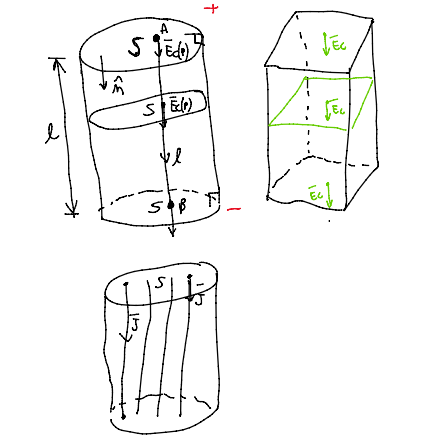
\includegraphics[scale = 0.5]{immagini/image11.png}
\end{center}
Si prende il provino e si seziona in superfici tutti uguali e piane, i campi quindi risultano uniformi all'interno del provino.
\[
u = \int_{A,l}^{B} \vec{E}_c \cdot \hat{t}  \, dl = \int_{A,l}^{B} |\vec{E}_c| \cdot \frac{\vec{E}_c}{|\vec{E}_c|} \cdot \hat{t}  \, dl = |\mathbf{E}_c|  \int_{A,l}^{B}\hat{u}\cdot\hat{t}dl = |\vec{E}_c|\cdot l
\]
\[
i = \int_S \vec{J}\cdot\hat{n} \, ds = |\vec{J}|\cdot S
\]
Sostituendo si arriva a dire che
\[
    \vec{E}_c = \rho\vec{J}
\]

\subsection*{Applicazioni dell'effetto Joule}

Si sfrutta per il riscaldamento: stufe a filo (non pompa di calore), piastra della cucina elettrica (non a induzione).

Nella maggior parte dei casi però l'effetto Joule è indesiderato perché provoca il riscaldamento dell'elettronica e dei fili percorsi da corrente. Questo produce due problemi:

1) Potenza dissipata inutile
2) Se il calore non viene dissipato, la temperatura aumenta. Questo è un problema molto grave che non permette l'ulteriore riduzione delle dimensioni dell'elettronica.

\subsection{Superfici di discontinuità della resistività}
\begin{center}
    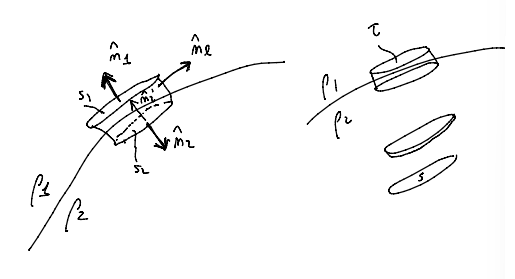
\includegraphics[scale = 0.6]{immagini/image12.png}
\end{center}
Si considera un volume $\tau$ a cavallo dell'interfaccia, S1,S2 sono le superfici "tappo" e le prendiamo uguali e infinitesime. La superficie laterale di $\tau$ è un infinitesimo di ordine superiore rispetto a S quindi risulta trascurabile.

\[
\int_{S1} \vec{J_1}\cdot\hat{n}_1 \, ds + \int_{S2} \vec{J_2}\cdot\hat{n}_1 \, ds + \cancel{\int_{Sl} \vec{J_l}\cdot\hat{n}_l \, ds} = -\frac{d}{dt}\int_S\sigma_cds
\]     
Per il principio di uniformità:
\[
    \vec{J}_1\cdot\hat{n}_1\cancel S + \vec{J}_2\cdot\hat{n}_2\cancel S = -\frac{\partial \sigma_c}{\partial t}\cancel S
\]
cambiando il riferimento per il secondo termine (cambio il segno) si ottiene alla fine che se
\[
-\frac{\partial \sigma_c}{\partial t} = 0 \Rightarrow \vec{J}_1\cdot\hat{n}_1 = \vec{J}_2\cdot\hat{n}_2'
\]

Si può fare il caso analogo prendendo una linea chiusa e ripetere il procedimento con il campo Elettrostatico. Si arriva a dedurre che: $\vec{E}_{C1} \cdot \hat{t}_1 = \vec{E}_{C2} \cdot \hat{t}_2$